\documentclass[12pt,english]{article}

\usepackage[utf8]{inputenc}

% bibliography stuff
%\usepackage[numbers]{natbib}
\usepackage[backend=biber,style=numeric]{biblatex}
%\usepackage{biblatex}
\addbibresource{references.bib}

\usepackage{graphicx}
\usepackage[margin=0.67in]{geometry}
\usepackage[en-US,useregional]{datetime2}
\usepackage{float}
\usepackage{xcolor}
\definecolor{linkblue}{HTML}{1F77B4}
\usepackage[colorlinks=true, allcolors=linkblue]{hyperref}
%\usepackage[colorlinks=true, linkcolor=linkblue, urlcolor=linkblue, citecolor=linkblue]{hyperref}
%\usepackage[urlcolor=linkblue, citecolor=linkblue]{hyperref} % still draws a box around the ref links
\usepackage{url}

\usepackage{amsmath}
\usepackage{amssymb}
\usepackage{mathtools}


\newenvironment{fixmathspace}{\abovedisplayskip=0pt\abovedisplayshortskip=0pt\belowdisplayskip=0pt\belowdisplayshortskip=0pt\vspace{-\baselineskip}}{}


\title{Harmonic Characterization of Musical Audio}
\author{Jesse Hautala\\ \href{mailto:hautala.j@northeastern.edu}{hautala.j@northeastern.edu}}
\date{2024-02-06}

\begin{document}

\maketitle

\begin{abstract}
This project aims to synthesize various techniques for musical audio signal processing into a hierarchical feature extraction pipeline, including note extraction, chord detection, and topic analysis from a corpus of musical pieces. The ultimate goal is to develop a robust system for song similarity search, music categorization, and playlist generation, on the basis of intrinsic features of musical audio data.
\end{abstract}

\section{Introduction}
\subsection{Background}
Audio signal processing, particularly in music, is a challenging yet rewarding field. The ability to understand and categorize music computationally opens numerous possibilities for music recommendation, generation, and analysis. Advanced tools like Melodyne have set a high standard in the industry for note extraction and manipulation, offering detailed segmentation of notes and their harmonics alongside a suite of editing capabilities (e.g. pitch, vibrato, amplitude, and duration).
\newline

\noindent
This project aims to identify and utilize existing open source tools that are well suited to hierarchical feature extraction and provide a novel and intuitive solution for navigating a music library. While Melodyne offers a remarkable capacity for note extraction and manipulation, our goal is to achieve a similar level of precision in note extraction within an open source framework, focusing primarily on the extraction aspect rather than the manipulation of audio signals. We will proceed to build higher-level features from there and hopefully discover meaningful patterns through the lens of western harmony.

\subsection{Problem Statement}
The project focuses on the extraction of musical features from complex audio signals, the detection of chords, and the analysis of musical corpora. Despite the advancements in deep learning for audio processing, achieving high accuracy in tasks like note extraction and song similarity search remains challenging, especially in the context of complex musical compositions.
\newline

\noindent
As a matter of expedience, this initial work is primarily focused on western ``functional harmony'' in the context of a twelve tone equal-tempered tuning system. Hopefully some of the tools and techniques explored and developed in the scope of this project will also be extensible to a more comprehensive analytical framework.

% !TEX root = proposal.tex

\section{Literature Review (Related Works)}

\subsection{General Overview}
A few key works provide the foundation for our understanding of the state of the art:
\begin{itemize}
    \item Y. Bayle's compilation of resources \cite{Bayle2018} offers an extensive list of deep learning techniques applied to music, only recently transitioning to unmaintained status (around \href{https://github.com/ybayle/awesome-deep-learning-music/commit/b252aaf8d441173d4b23bcdd184f2d2fcd61d7cb#diff-b335630551682c19a781afebcf4d07bf978fb1f8ac04c6bf87428ed5106870f5R1}{2023-12-15}).
    \item H. Purwins et al. \cite{Purwins2019} provide a comprehensive overview of deep learning applications in audio signal processing.
    \item Parekh et al. \cite{parekh2022listen} addresses interpretability of NN solutions, utilizing non-negative matrix factorization (NMF).
\end{itemize}

\subsection{Reference Annotations and Tools}
To inform the process of generating annotations for notes and chords, we will review extant annotation schemas, including the Reference Annotations of the Centre for Digital Music \cite{IsophonicsReferenceAnnotations}, particularly the \textit{Reference Annotations: The Beatles} \cite{ReferenceAnnotationsBeatles} metadata.

\subsection{Note Extraction}
\begin{itemize}
	\item Bay et al. \cite{bay2009evaluation} compare multiple techniques in \textit{Evaluation of multiple-f0 estimation and tracking systems}.
	\item In one of the older papers we came across, Tolonen and Karjalainen \cite{tolonen2000computationally} present an efficient technique.
	\item In another older paper, also focused on efficiency, Klapuri \cite{klapuri2006multiple} introduces the ``salience spectrum''.
	\item Barbedo at al. \cite{barbedo2007high} extend Klapuri's work, in an iterative manner, that seems intuitive to me.
	\item Heittola et al. \cite{heittola2009musical} introduce non-negative matrix factorization (or NMF).
	\item Bittner et al. \cite{bittner2017deep} introduce deep learning methods.
	\item In a more recent work, Won et al. \cite{won2020data} use a ``harmonic filter'' in front of a convolutional neural net.
	\item Mariotte et al. \cite{mariotte2024explainable} perform comprehensive audio segmentation, again also using NMF, but not limited to musical audio (perhaps a bit too general, but involving interesting techniques).
	\item Perhaps a bit specific for our purposes, Gómez et al. \cite{gomez2012predominant} approach fundamental extraction for flamenco vocals in the context of guitar accompaniment (so, a bit more complex than a monophonic sound source, but not as complex as arbitrary full ensemble context).
\end{itemize}

\newpage
\subsection{Chord Detection}
\begin{itemize}
	\item Mauch et al. \cite{mauch2010approximate} focus on improving recognition of particularly challenging chords.
	\item Jacoby et al. \cite{jacoby2015information} address many different encodings for functional harmonic concepts (e.g. function theory, root theory, and figured bass).
	\item De Haas et al. \cite{de2011harmtrace} introduce the \textsc{HarmTrace} system of chord labeling.
	\item I have not worked out how to access the paper yet but Magalhaes and De Haas \cite{magalhaes2011functional} report that they developed a powerful Haskell model for harmonic analysis.
\end{itemize}


% !TEX root = proposal.tex

\section{Methodology (Proposed Algorithms)}
This section outlines the steps and algorithms proposed for the audio signal processing project, focusing on feature extraction, similarity metrics, and applications.

\subsection{Feature Extraction}
At a high level, we aim to accomplish the following hierarchical feature extraction:
\begin{quote}
\begin{fixmathspace}
\begin{flalign*}
    \text{raw audio} &\rightarrow \text{frequencies/tones (e.g. via FFT)}&&\\
    &\rightarrow \text{fundamentals/notes}&&\\
%    &\rightarrow \text{key, reference pitch (TBD)}&&\\
    &\rightarrow \text{functional harmony/chords and sequences}&&\\
    &\rightarrow \text{topics/genres (e.g. via LDA)}
\end{flalign*}
\end{fixmathspace}
\end{quote}

\begin{enumerate}
    \item In order to extract notes, we analyze harmonic information to identify fundamental tones. We may be able to distinguish them from overtones based on the quirks of equal tempered tuning (see Figure $\ref{fig:12tet_spiral}$ for a visualization of the discrepancy between 12-tet and pure harmonics). We will likely require high resolution on the frequency axis, if we are to distinguish between natural harmonics and tempered tones. If high resolution Short-Time Fourier Transform algorithms are prohibitively slow, perhaps we can use QISP \cite{Smith2011}. See Figure $\ref{fig:qisp}$ for some preliminary test results, rendered in a custom visualization we developed for comparing spectrograms to a musical scale.
    \item From note information, we can infer the key and reference pitch, to provide context for the harmonic information. These may be useful metadata in themselves for other processes, but in this pipeline we expect they will mainly be ``factored out'' so we can focus on functional harmony independently.
    \item Given a collection of notes, we can analyze intervalic relationships to derive harmonic functions and identify chords, which will be the primary terms in our subsequent analysis. A degree of reductionism is inherent in functional analysis; our selection of how to encode chordal information will largely determine the capacity of models to detect similarities and differentiate pieces of music.
    \item Finally, we can analyze all the chords and sequences thereof in a corpus, to perform topic extraction. Such high-level features can be used in subsequent calculation of similarity metrics between pieces of music and similarity-based search functions.
\end{enumerate}

\begin{figure}[H]
    \centering
    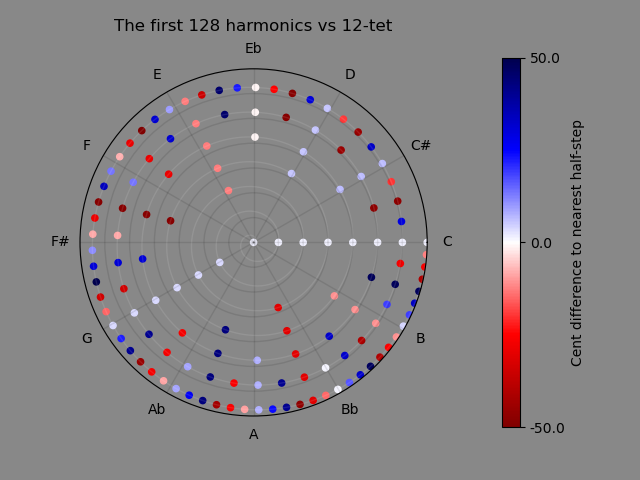
\includegraphics[scale=0.67]{12tet_spiral.png}
    \caption{An illustration of the relationship between equal tempered tuning and natural harmonics}
    \label{fig:12tet_spiral}
\end{figure}

\begin{figure}[H]
    \centering
    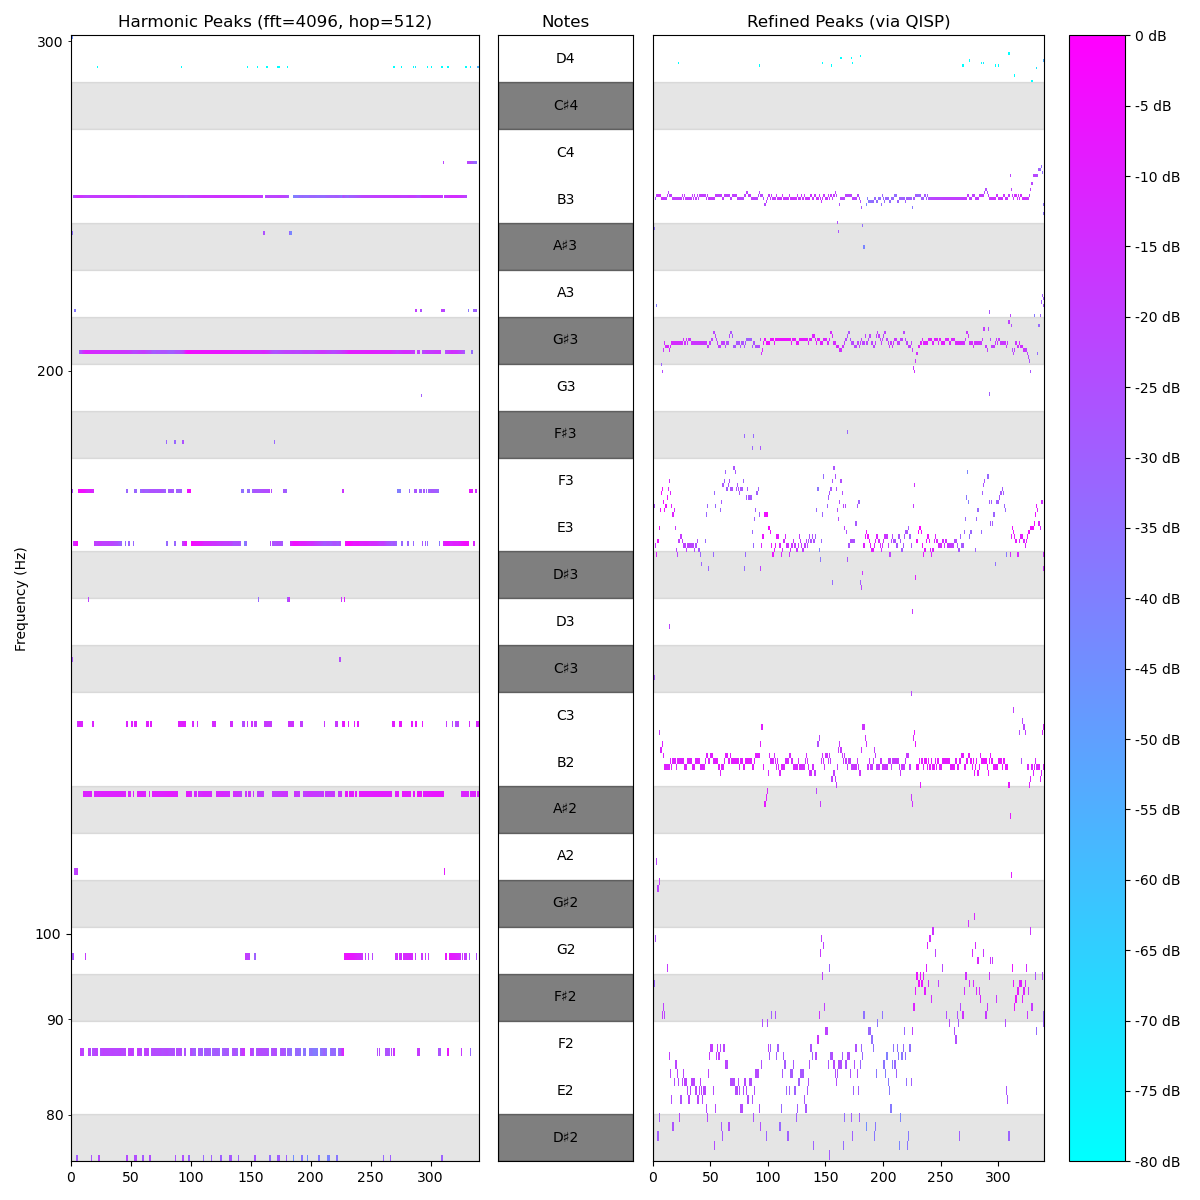
\includegraphics[scale=0.40]{qisp.png}
    \caption{Lower notes (e.g. B2) are particularly susceptible to quantization error}
    \label{fig:qisp}
\end{figure}

\newpage
\subsection{Similarity Metrics}
To compare different pieces of music and identify similarities, we will employ various metrics such as Cosine Similarity, TFIDF, and market basket analysis metrics (e.g. Jaccard Index).

\subsection{Applications}
The extracted features and similarity metrics can be utilized in several applications:
\begin{itemize}
    \item Audio playback and visualization of extracted features.
    \item Implementation of a search by similarity/dissimilarity feature.
    \item Automated playlist creation based on the similarity of songs.
\end{itemize}

\subsection{Challenges}
The primary challenge anticipated is the ambiguity prevalent in various stages, from fundamental detection to chord assignment. This work will focus on functional harmony in the context of a twelve-tone equal-tempered tuning system, aiming for extensibility to a broader analytical framework in future developments.


\section{Data Collection Plan}
Assuming we can obtain access to the correct raw audio data, we would prefer to utilize community datasets such as the Million Song Dataset \cite{MillionSongDataset}, MagnaTagATune \cite{MagnaTagATune}, and MTG-Jamendo \cite{MTGJamendo}. These datasets offer a rich collection of songs and associated metadata, which could be useful for training and evaluating the proposed models. If we are unable to obtain a coherent corpus from community sources, our backup plan is to use audio data from personal collections, consisting of original recordings in WAV format and backup copies of commercial audio CDs in MP3 format.

\begin{itemize}
    \item The Million Song Dataset \cite{MillionSongDataset} is a rich collection of audio features and metadata for a substantial number of songs. Obtaining the corresponding raw audio data may prove to be a significant challenge.
    \item MagnaTagATune provides a collection of music and annotations that should be amenable to the aims of this project, being offered by City University of London, under the Creative Commons Attribution – Noncommercial-Share Alike 3.0 license.
    \item MTG-Jamendo also provides a large collection of labeled music under various Creative Commons licenses.
\end{itemize}

\section{Evaluation Plan}
We will implement various forms of ad hoc, manual validation to qualitatively assess the relevance of final results. For example, in the context of note and chord extraction we can use our ears, musical instruments, and any extant musical transcriptions to assess accuracy, but to a large extent this development plan is in the domain of unsupervised learning. Where we have ground truth, we can compare our model against random, so-called ``null'' models, to assess whether it produces results that are better than guessing.

%\section{Project Plan}
%
%something?

%\section{Conclusion and Discussion}
%The project aims to push the boundaries of current music processing techniques. By implementing and evaluating various algorithms, the project seeks to offer insights into the complexities of musical audio processing and contribute to the field of music information retrieval.

%\bibliographystyle{plainnat}
%\bibliography{references}
%\printbibliography[heading=bibintoc, title={References}]
\printbibliography

\end{document}
